% !TeX root = ../main.tex
\begin{figure*}[t]
\centering
\ifdefined\OverviewDataBenchmark
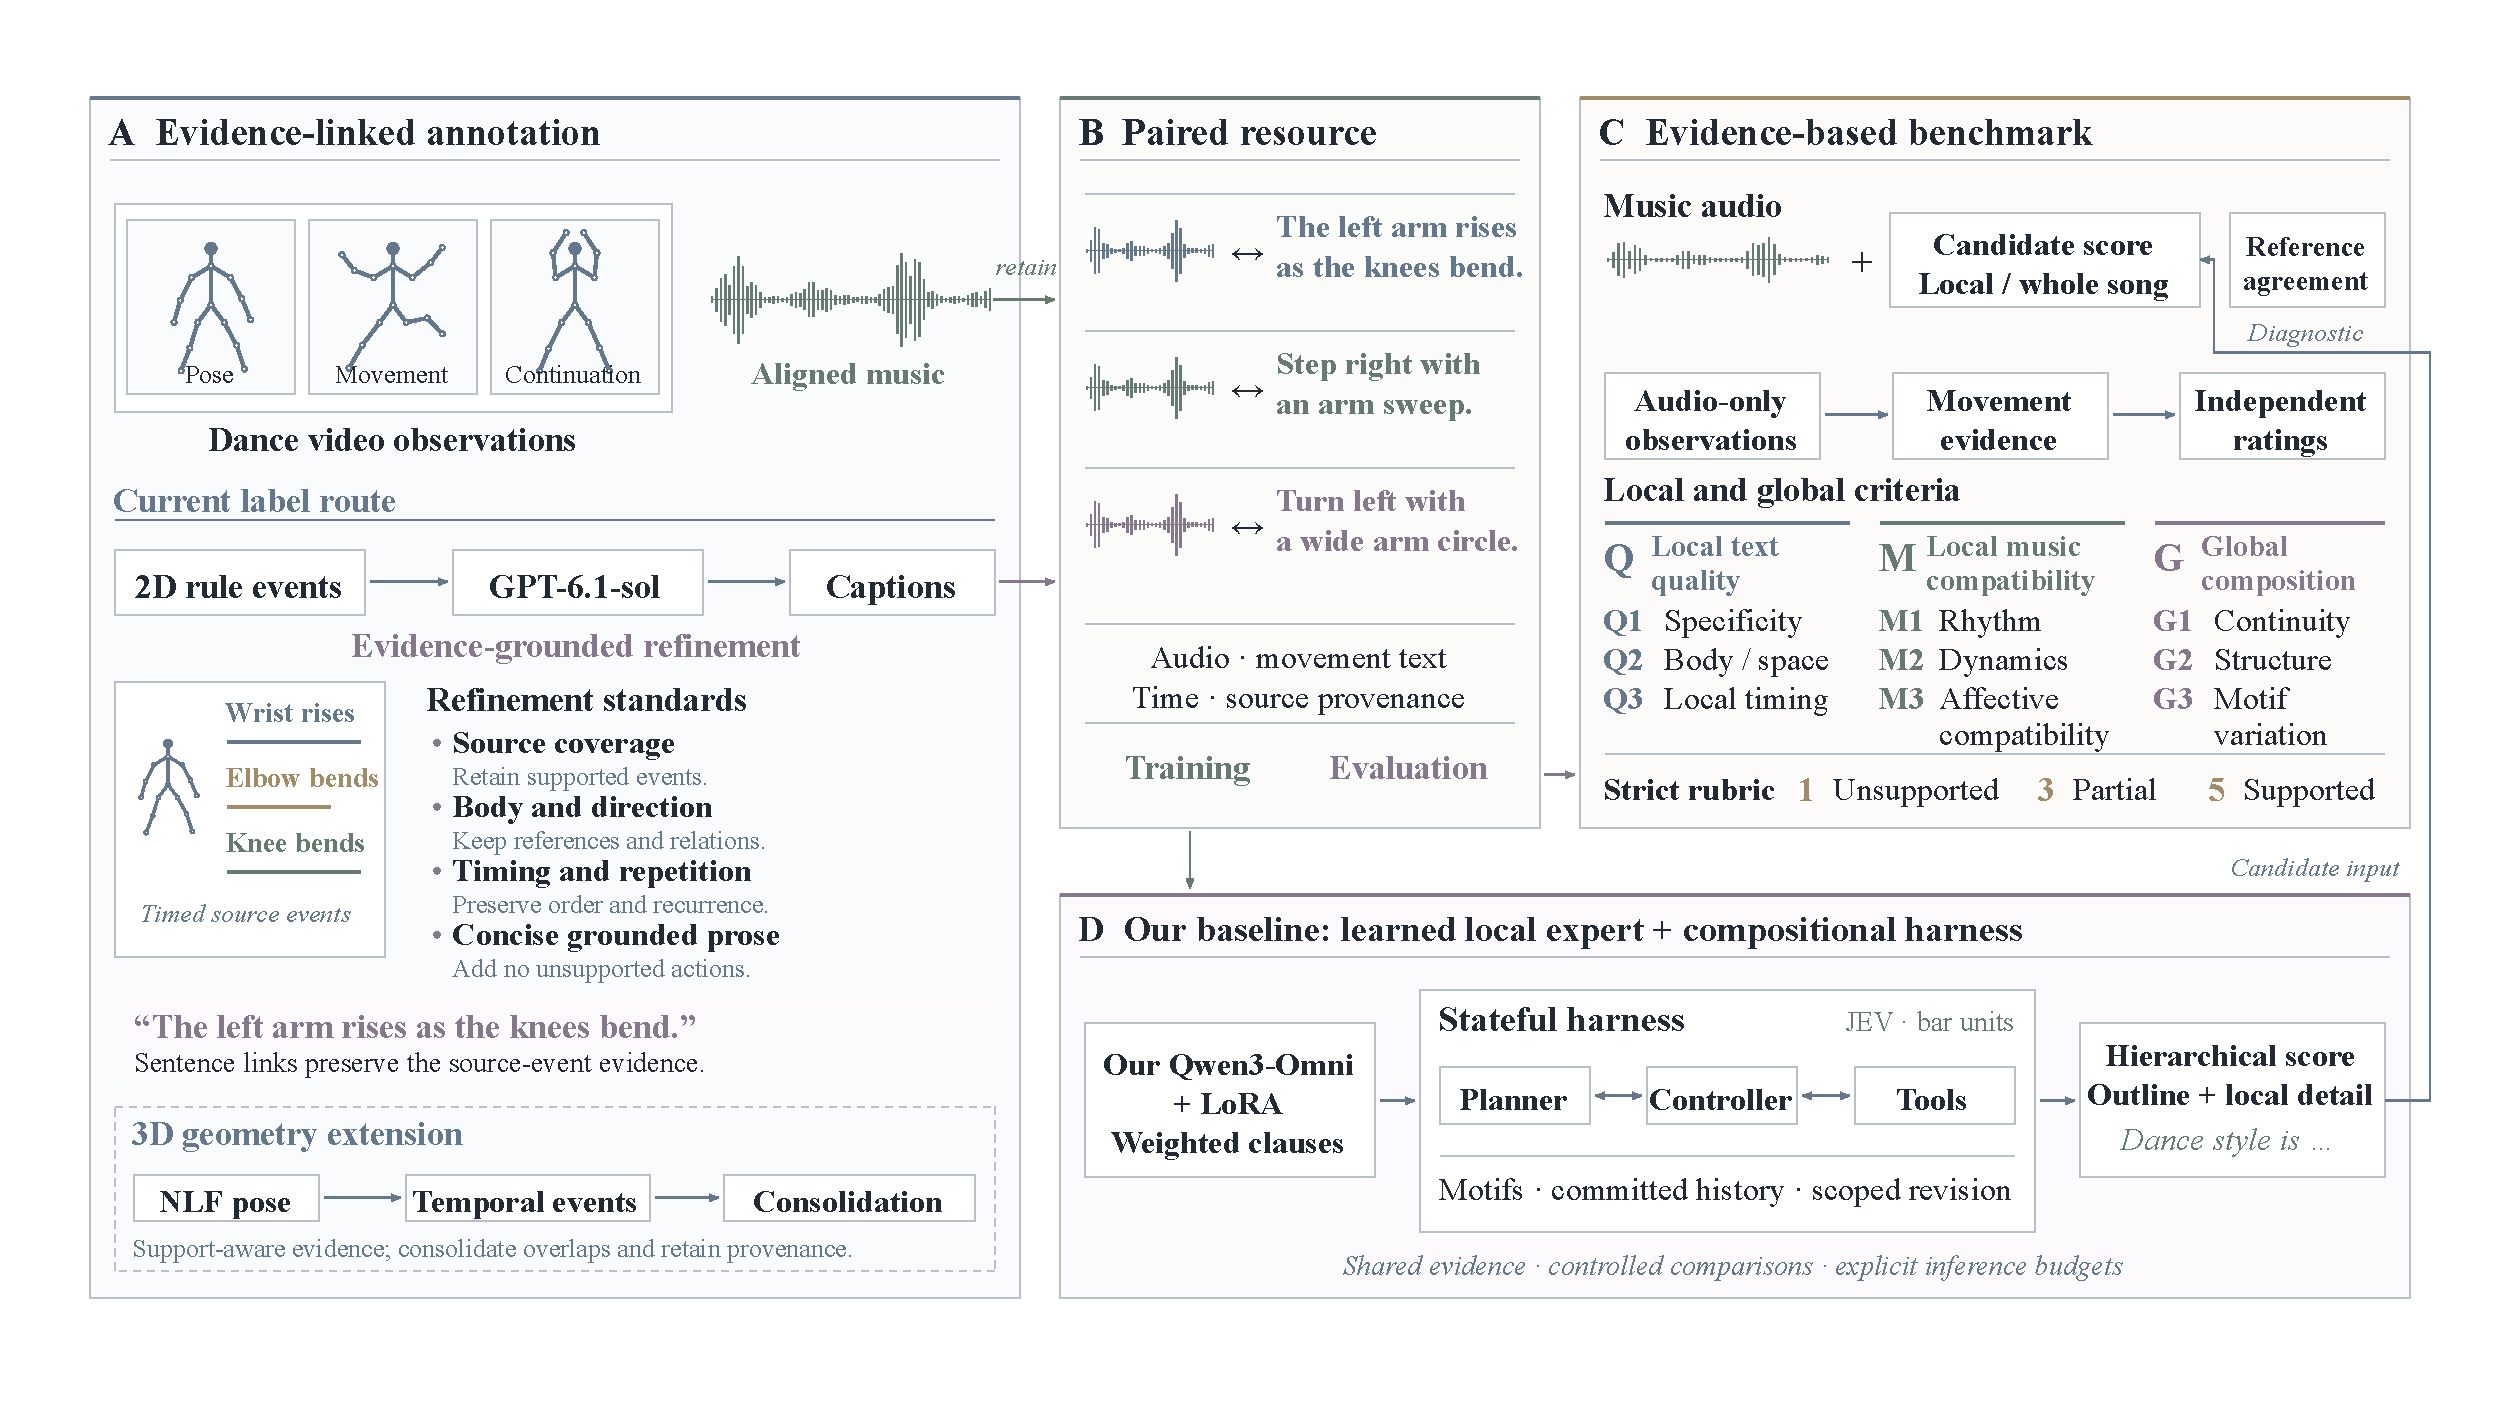
\includegraphics[width=\textwidth]{figures/revision_20261117/paper/overview_benchmark.pdf}
\caption{\textbf{Data, benchmark, and baseline in \method.}
Evidence-linked captions retain movement provenance and paired music.
Current labels follow the 2D rule-event route; the dashed 3D route
depicts the geometry extension. The trained local expert and stateful
harness provide a baseline for assessing local movement, musical
response, and whole-song composition. The proposed protocol uses audio
and quoted movement evidence; calibration remains pending.
Media, score snippets, and rubric anchors are schematic illustrations.}
\else
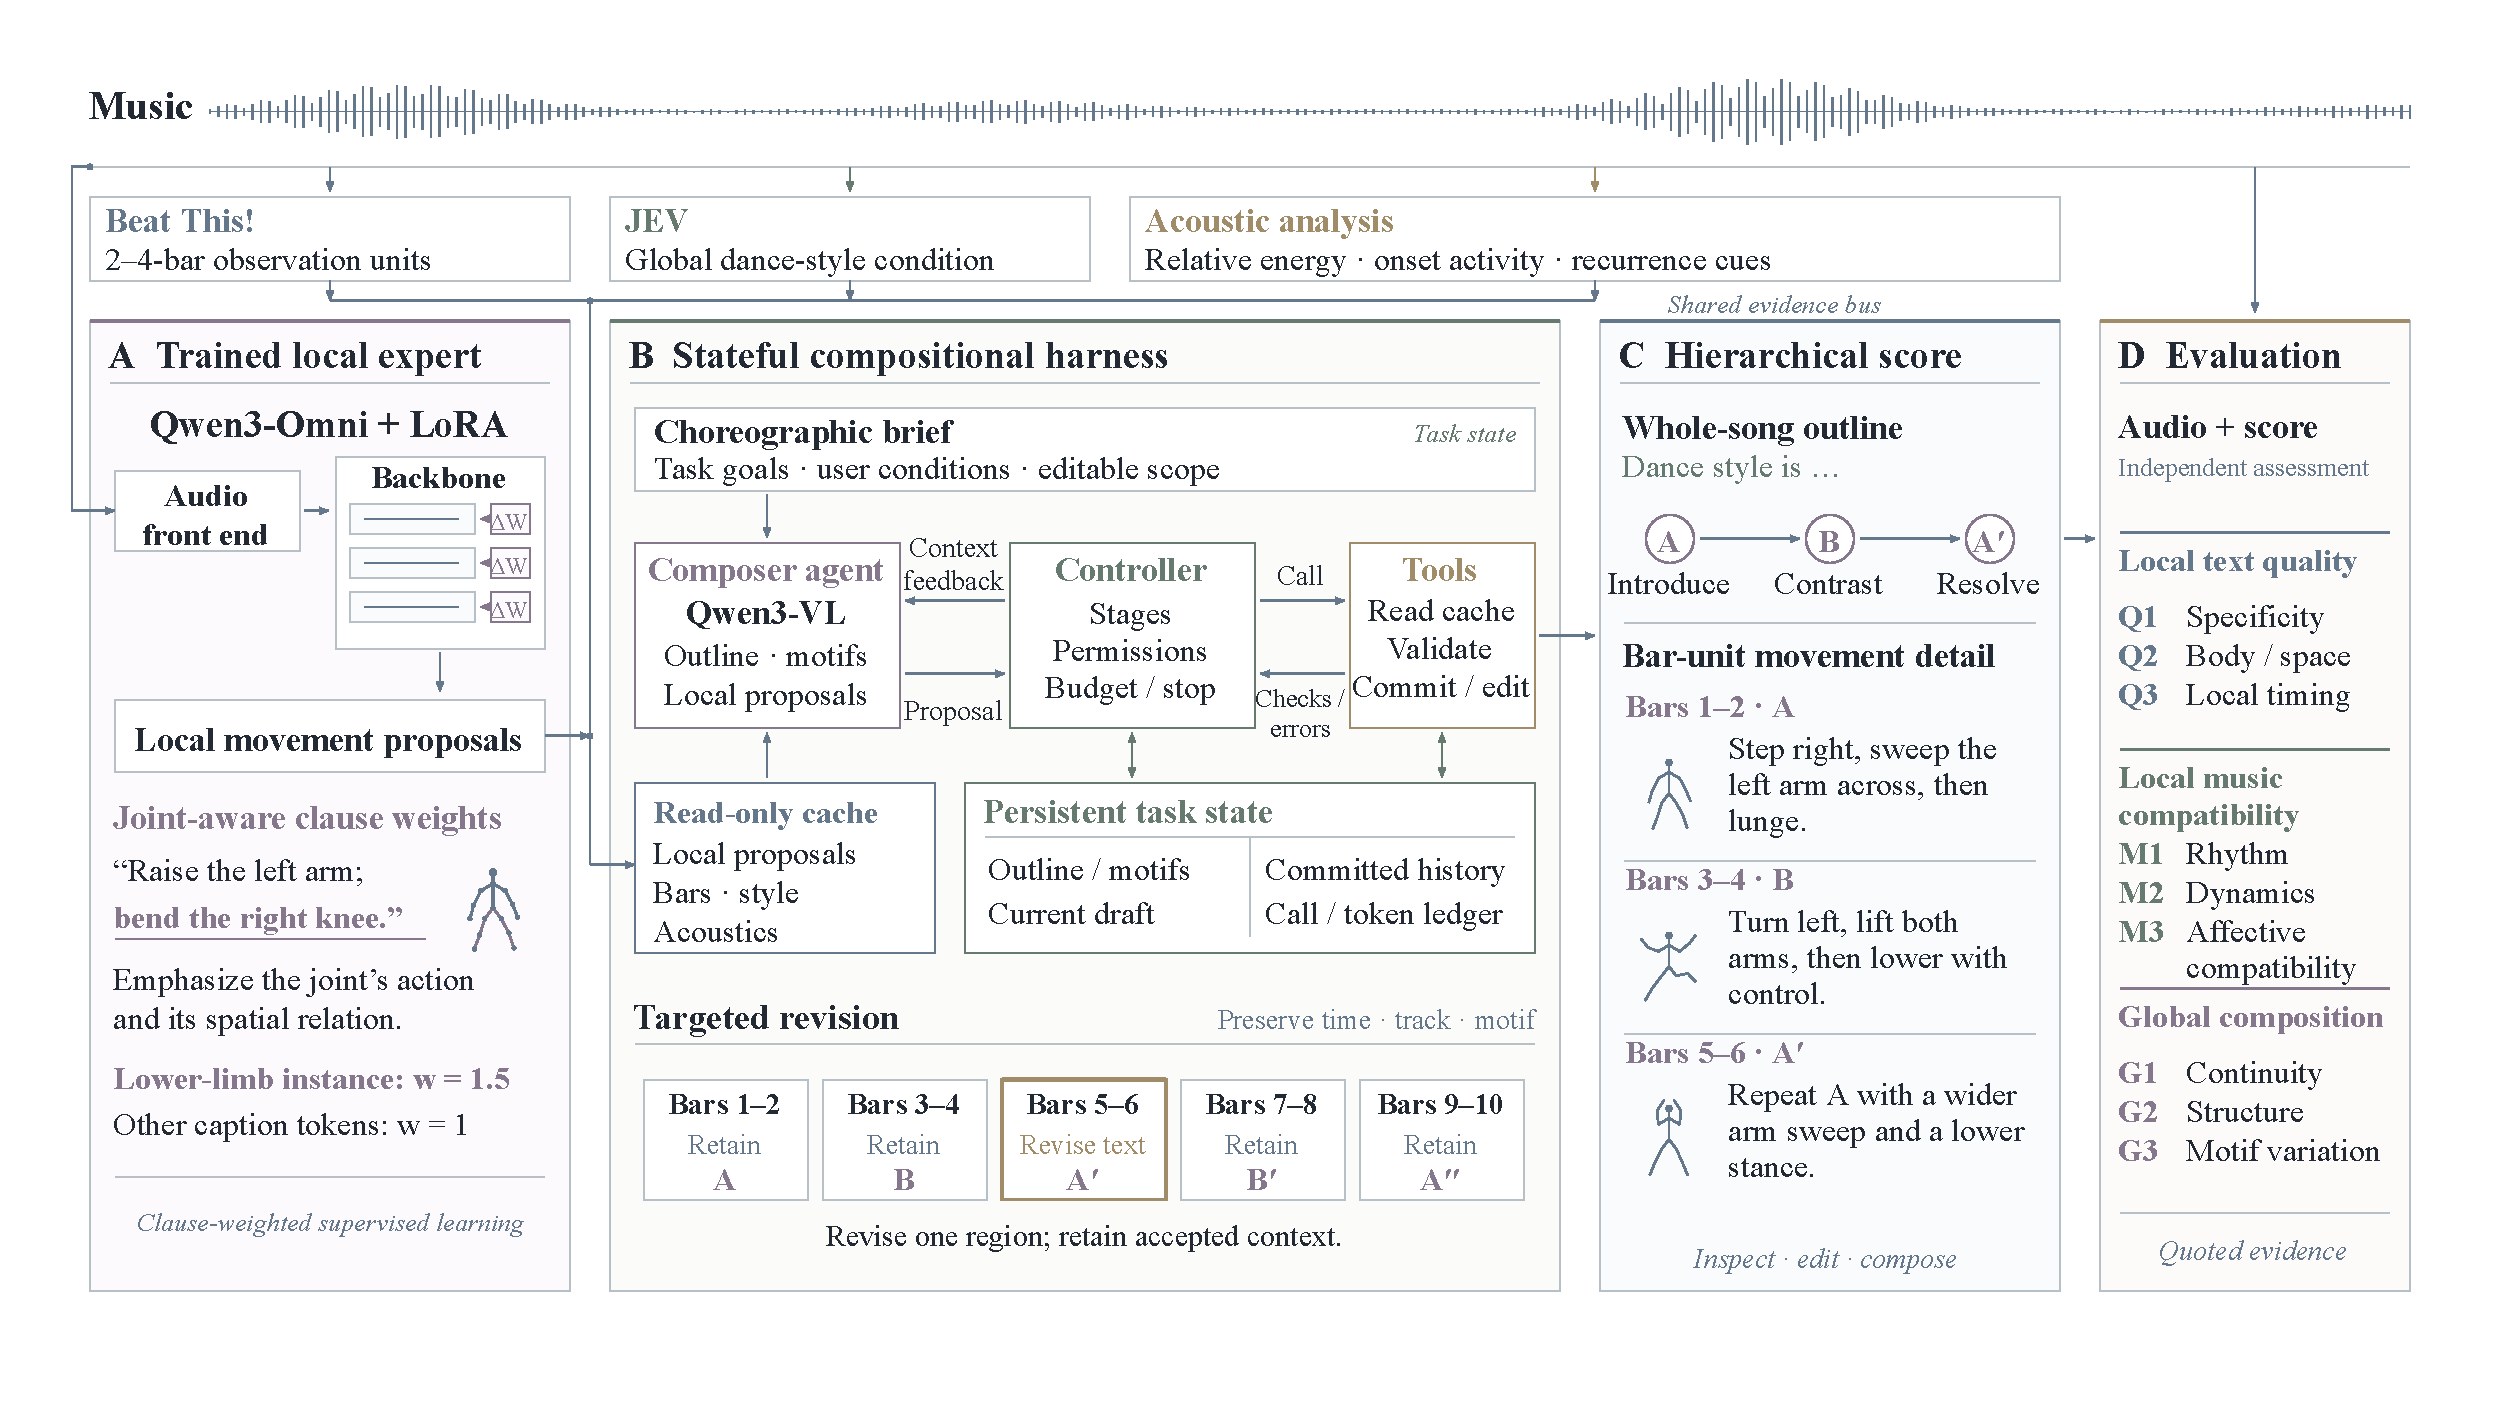
\includegraphics[width=\textwidth]{figures/revision_20261117/paper/overview_method.pdf}
\caption{\textbf{From a trained local expert to stateful composition.}
Joint-aware clause supervision trains our Qwen3-Omni expert; Beat This!,
JEV, and acoustic analysis provide shared musical conditions.
The composer proposes movements, the controller schedules tool
execution, and structural feedback informs subsequent decisions.
The task brief and persistent state retain objectives, drafts, motifs,
committed history, and budgets.
Targeted revision protects the temporal scaffold and accepted context.
The hierarchical score supports separate local and global assessment
outside the generation loop. Poses and score excerpts are schematic. The latest design uses bar
groups; reported whole-song results retain their fixed-window configuration.}
\fi
\label{fig:harness-overview}
\end{figure*}
